% Gerado automaticamente. No preambulo do documento use:
% \usepackage{pgfplots}
% \pgfplotsset{compat=1.18}
\definecolor{plotblue}{HTML}{2563EB}
\definecolor{plotorange}{HTML}{D97706}
\definecolor{plotgreen}{HTML}{059669}
\definecolor{plotpurple}{HTML}{7C3AED}
\definecolor{plotgray}{HTML}{374151}
\definecolor{plotred}{HTML}{DC2626}
\definecolor{plotteal}{HTML}{0F766E}
\definecolor{plotslate}{HTML}{64748B}

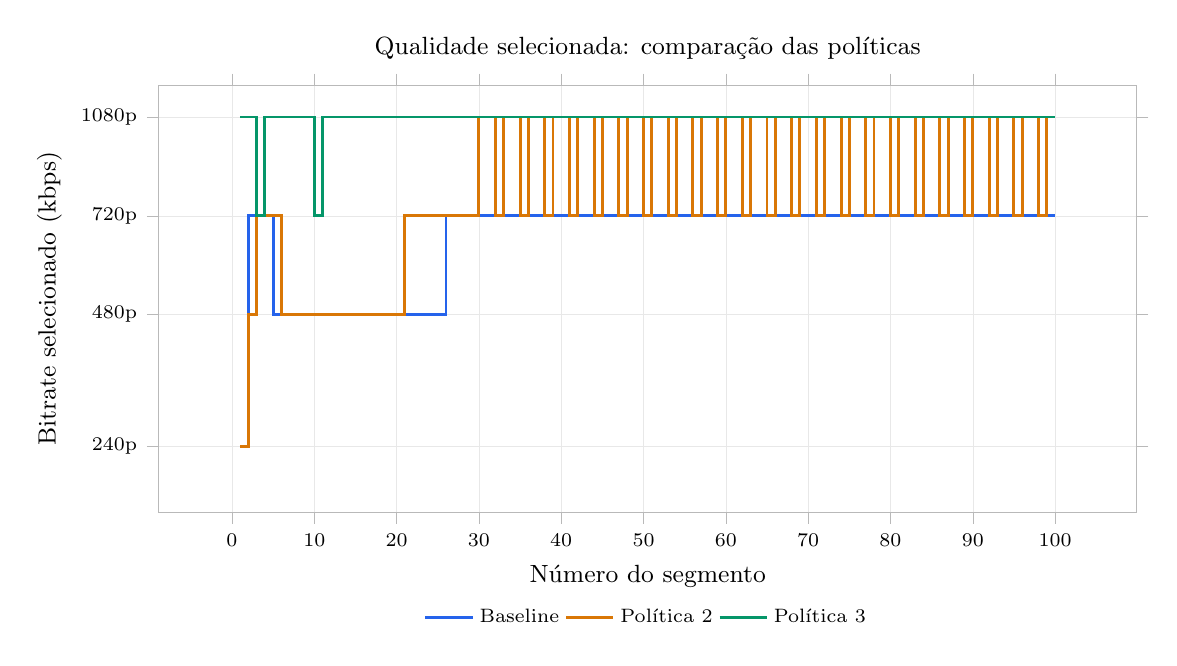
\begin{tikzpicture}
\begin{axis}[
    title={Qualidade selecionada: comparação das políticas},
    xlabel={Número do segmento},
    ylabel={Bitrate selecionado (kbps)},
    width=14cm,
    height=7cm,
    grid=major,
    grid style={line width=.12pt, draw=gray!18},
    axis line style={draw=gray!55},
    tick style={draw=gray!55},
    tick align=outside,
    title style={font=\small},
    label style={font=\small},
    tick label style={font=\scriptsize},
    legend cell align={left},
    legend style={at={(0.5,-0.20)}, anchor=north, legend columns=3, draw=none, font=\scriptsize},
    ymin=0,
    ymax=1296,
    ytick={200,600,900,1200},
    yticklabels={{240p},{480p},{720p},{1080p}}
]
\addplot+[plotblue, const plot, line width=1.05pt, mark=none] coordinates {
(1,200)
(2,900)
(3,900)
(4,900)
(5,600)
(6,600)
(7,600)
(8,600)
(9,600)
(10,600)
(11,600)
(12,600)
(13,600)
(14,600)
(15,600)
(16,600)
(17,600)
(18,600)
(19,600)
(20,600)
(21,600)
(22,600)
(23,600)
(24,600)
(25,600)
(26,900)
(27,900)
(28,900)
(29,900)
(30,900)
(31,900)
(32,900)
(33,900)
(34,900)
(35,900)
(36,900)
(37,900)
(38,900)
(39,900)
(40,900)
(41,900)
(42,900)
(43,900)
(44,900)
(45,900)
(46,900)
(47,900)
(48,900)
(49,900)
(50,900)
(51,900)
(52,900)
(53,900)
(54,900)
(55,900)
(56,900)
(57,900)
(58,900)
(59,900)
(60,900)
(61,900)
(62,900)
(63,900)
(64,900)
(65,900)
(66,900)
(67,900)
(68,900)
(69,900)
(70,900)
(71,900)
(72,900)
(73,900)
(74,900)
(75,900)
(76,900)
(77,900)
(78,900)
(79,900)
(80,900)
(81,900)
(82,900)
(83,900)
(84,900)
(85,900)
(86,900)
(87,900)
(88,900)
(89,900)
(90,900)
(91,900)
(92,900)
(93,900)
(94,900)
(95,900)
(96,900)
(97,900)
(98,900)
(99,900)
(100,900)
};
\addlegendentry{Baseline}
\addplot+[plotorange, const plot, line width=1.05pt, mark=none] coordinates {
(1,200)
(2,600)
(3,900)
(4,900)
(5,900)
(6,600)
(7,600)
(8,600)
(9,600)
(10,600)
(11,600)
(12,600)
(13,600)
(14,600)
(15,600)
(16,600)
(17,600)
(18,600)
(19,600)
(20,600)
(21,900)
(22,900)
(23,900)
(24,900)
(25,900)
(26,900)
(27,900)
(28,900)
(29,900)
(30,1200)
(31,1200)
(32,900)
(33,1200)
(34,1200)
(35,900)
(36,1200)
(37,1200)
(38,900)
(39,1200)
(40,1200)
(41,900)
(42,1200)
(43,1200)
(44,900)
(45,1200)
(46,1200)
(47,900)
(48,1200)
(49,1200)
(50,900)
(51,1200)
(52,1200)
(53,900)
(54,1200)
(55,1200)
(56,900)
(57,1200)
(58,1200)
(59,900)
(60,1200)
(61,1200)
(62,900)
(63,1200)
(64,1200)
(65,900)
(66,1200)
(67,1200)
(68,900)
(69,1200)
(70,1200)
(71,900)
(72,1200)
(73,1200)
(74,900)
(75,1200)
(76,1200)
(77,900)
(78,1200)
(79,1200)
(80,900)
(81,1200)
(82,1200)
(83,900)
(84,1200)
(85,1200)
(86,900)
(87,1200)
(88,1200)
(89,900)
(90,1200)
(91,1200)
(92,900)
(93,1200)
(94,1200)
(95,900)
(96,1200)
(97,1200)
(98,900)
(99,1200)
(100,1200)
};
\addlegendentry{Política 2}
\addplot+[plotgreen, const plot, line width=1.05pt, mark=none] coordinates {
(1,1200)
(2,1200)
(3,900)
(4,1200)
(5,1200)
(6,1200)
(7,1200)
(8,1200)
(9,1200)
(10,900)
(11,1200)
(12,1200)
(13,1200)
(14,1200)
(15,1200)
(16,1200)
(17,1200)
(18,1200)
(19,1200)
(20,1200)
(21,1200)
(22,1200)
(23,1200)
(24,1200)
(25,1200)
(26,1200)
(27,1200)
(28,1200)
(29,1200)
(30,1200)
(31,1200)
(32,1200)
(33,1200)
(34,1200)
(35,1200)
(36,1200)
(37,1200)
(38,1200)
(39,1200)
(40,1200)
(41,1200)
(42,1200)
(43,1200)
(44,1200)
(45,1200)
(46,1200)
(47,1200)
(48,1200)
(49,1200)
(50,1200)
(51,1200)
(52,1200)
(53,1200)
(54,1200)
(55,1200)
(56,1200)
(57,1200)
(58,1200)
(59,1200)
(60,1200)
(61,1200)
(62,1200)
(63,1200)
(64,1200)
(65,1200)
(66,1200)
(67,1200)
(68,1200)
(69,1200)
(70,1200)
(71,1200)
(72,1200)
(73,1200)
(74,1200)
(75,1200)
(76,1200)
(77,1200)
(78,1200)
(79,1200)
(80,1200)
(81,1200)
(82,1200)
(83,1200)
(84,1200)
(85,1200)
(86,1200)
(87,1200)
(88,1200)
(89,1200)
(90,1200)
(91,1200)
(92,1200)
(93,1200)
(94,1200)
(95,1200)
(96,1200)
(97,1200)
(98,1200)
(99,1200)
(100,1200)
};
\addlegendentry{Política 3}
\end{axis}
\end{tikzpicture}
